\section{Chapter 12}

\begin{itemize}

      \item[R-12.3] List the prefixes of the string P ="aaabbaaa" that are also suffixes of P.\\
            \answer \\
            "", "a", "aa", "aaa"
      \item [R-12.4] Draw a figure illustrating the comparisons done by brute-force pattern
            matching for the text "aaabaadaabaaa" and pattern "aabaaa". \\
            \answer \\
            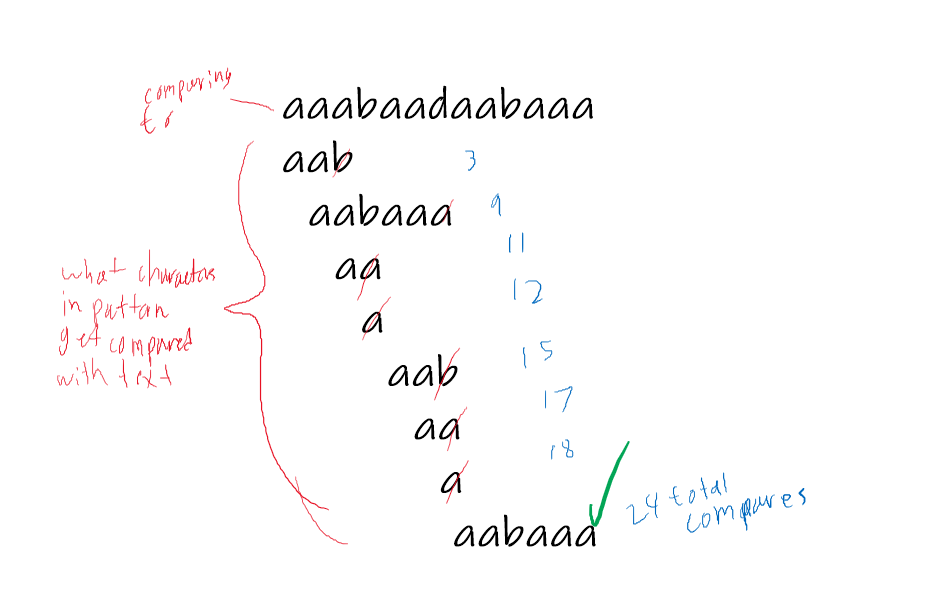
\includegraphics[scale = .6]{img/R-12_4.png}
      \item[R-12.5] Repeat the previous problem for the BM pattern matching algorithm, not
            counting the comparisons made to compute the last(c) function. \\
            \answer \\
            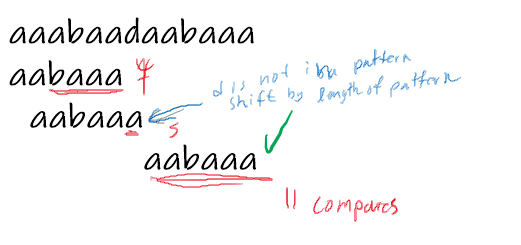
\includegraphics[scale = 0.6]{img/R-12_5.png}
            \newpage
      \item[R-12.6] Repeat the previous problem for the KMP pattern matching algorithm, not
            counting the comparisons made to compute the failure function.\\
            \answer \\
            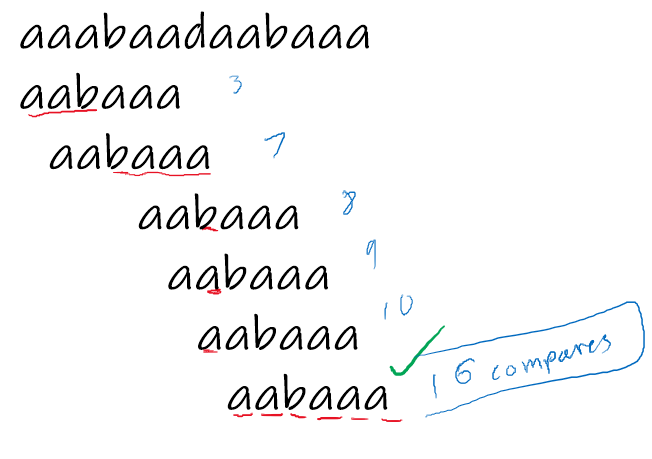
\includegraphics[scale = 0.6]{img/R-12_6.png}
      \item[R-12.9] Compute a table representing the KMP failure function for the pattern
            string "cgtacgttcgtac".\\
            \answer \\
            \begin{tabular}{|*{13}{c|}}
                  \hline
                  c & g & t & a & c & g & t & t & c & g & t & a & c \\
                  \hline
                  0 & 0 & 0 & 0 & 1 & 2 & 3 & 0 & 1 & 2 & 3 & 4 & 5 \\
                  \hline
            \end{tabular}
      \item [R-12.10] Draw a standard trie for the following set of strings: \\
            \{abab, baba, ccccc, bbaaaa, caa, bbaacc, cbcc, cbca\}.\\
            \answer \\
            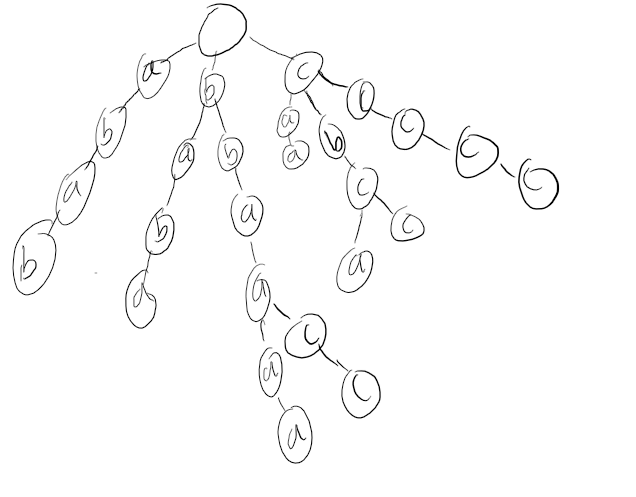
\includegraphics[scale = .7]{img/R-12_10.png}
            \newpage
      \item[R-12.11]Draw a compressed trie for the set of strings given in Exercise R-12.10.\\
            \answer \\
            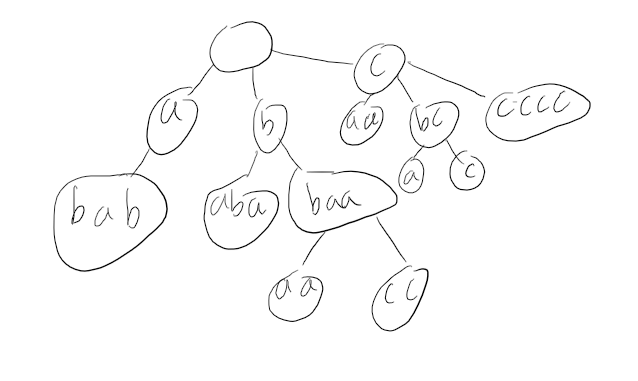
\includegraphics[scale=0.7]{img/R-12_11.png}
      \item [R-12.13] What is the longest prefix of the string "cgtacgttcgtacg" that is also a
            suffix of this string?\\
            \answer \\
            cgtacg
      \item[R-12.14] Draw the frequency array and Huffman tree for the following string:\\
            "dogs do not spot hot pots or cats".\\
            \answer \\
            \begin{tabular}{|*{13}{c|}}
                  \hline
                  Character &   & a & c & d & g & h & n & o & p & r & s & t \\
                  \hline
                  Frequency & 7 & 1 & 1 & 2 & 1 & 1 & 1 & 7 & 2 & 1 & 4 & 5 \\
                  \hline
            \end{tabular}
            \\
            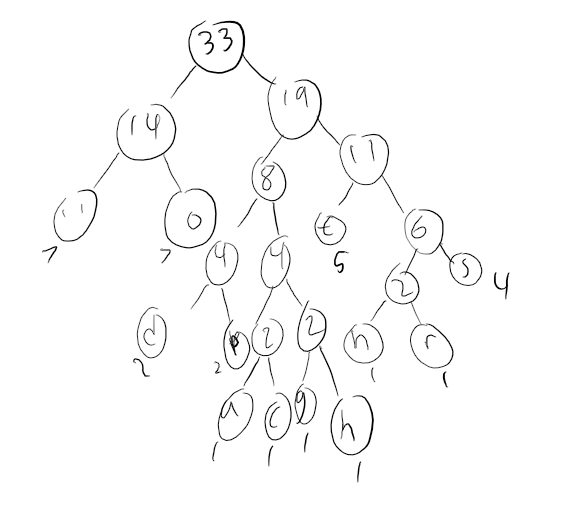
\includegraphics[scale = .7]{img/R-12_14.png}
      \item[C-12.1]  A native Australian named Anatjari wishes to cross a desert carrying only
            a single water bottle. He has a map that marks all the watering holes along
            the way. Assuming he can walk k miles on one bottle of water, design an
            efficient algorithm for determining where Anatjari should refill his bottle
            in order to make as few stops as possible. Argue why your algorithm is
            correct. \\
            \answer \\
            Use a greedy algorithm that chooses the watering hole that is the maximal distance
            still less than k miles. Do so until he reaches the end.

      \item[C-12.3] Give an example set of denominations of coins so that a greedy change-
            making algorithm will not use the minimum number of coins. \\
            \answer \\
            {25, 10, 1} to make 55 would use{25, 25, 1, 1, 1, 1, 1} but the optimal solution is {25, 10, 10, 10}.








\end{itemize}